\documentclass[12pt]{article}
\usepackage[margin=1in]{geometry}
\usepackage{times}
\usepackage{graphicx}
\usepackage{hyperref}
\usepackage{amsmath}
\usepackage{listings}
\usepackage{xcolor}
\usepackage{float}
\usepackage{caption}
\usepackage{subcaption}
\usepackage{booktabs}
\usepackage[numbers]{natbib}

\hypersetup{
    colorlinks=true,
    linkcolor=blue,
    urlcolor=blue,
    citecolor=blue,
}

\title{LLM Network Intrusion Detection System}
\author{
    INSyT (Innovative Network Security Technologies)\\
    Taeyang Kim, Bronze Frazer, Isaac Peterson, Damon Tingey\\
    \and
    Sandia National Laboratories\\
    Ryan Holt, Mike Reed\\
}

\date{}

\begin{document}

\maketitle

\begin{abstract}
Current network intrusion detection systems (NIDS) struggle to keep pace with the sophistication and evolving nature of cyberattacks. Traditional signature-based and rule-based systems are often brittle and easily bypassed, while anomaly-based systems suffer from high false positives. This leaves an alarming gap in network security, exposing organizations to data breaches, financial losses, and reputational damage.

We propose the development of a full-stack Large Language Model (LLM) product designed to revolutionize threat analysis through the comprehensive examination of system and network logs as natural language. This solution aims to provide systems that can understand complex attack protocols, detect novel attacks, and adapt to evolving threats. Our system enhances security with proactive and comprehensive defense against a wider range of threats, improves efficiency through accurate threat detection and reduced false positives, and offers a future-proofed defense with continuous adaptation to evolving threats, ensuring long-term effectiveness and protection against emerging attack vectors.
\end{abstract}

\section{Introduction}

Network intrusion refers to unauthorized access or activity on a computer network, often with malicious intent, such as stealing data or disrupting services. In 2023, the average cost per data breach in the United States was \$9,480,000 \citep{databreachreport}. Organizations face significant financial losses, operational disruptions, and reputational damage due to sophisticated cyberattacks that traditional NIDS struggle to detect effectively.

Current NIDS rely heavily on signature-based and rule-based methodologies, which are often inflexible and unable to detect novel or sophisticated attacks \citep{traditionalnids}. Anomaly-based systems, while more adaptive, tend to generate high false-positive rates, burdening security teams with excessive alerts \citep{anomalyissues}.

To address these challenges, we propose a novel approach: leveraging advanced LLMs to analyze system and network logs as natural language, enabling a deeper understanding of complex attack patterns and the detection of previously unseen threats.

\section{Related Work}

Machine learning has been applied to NIDS with varying degrees of success. Previous work has explored the use of neural networks for intrusion detection \citep{neuralnids}, but they often lack the ability to interpret the semantic content of log data effectively. Recent advancements in Natural Language Processing (NLP) and LLMs, such as BERT \citep{bert}, have shown promise in interpreting and classifying text data, which can be applied to system logs.

Our approach distinguishes itself by treating log data as a form of pseudo-natural language, allowing the LLM to learn patterns and correlations that traditional models may miss.

\section{The Data}

\subsection{Data Source}

We obtained our data from a research group in Australia that simulated attacks over a period of seven days on seven different servers \citep{landauer2022ait}. The dataset includes a wide variety of attack types and a substantial amount of system and network log entries.

\subsection{Data Imbalance}

A significant challenge with the data is the imbalance among the different classes. Figure~\ref{fig:label_counts} illustrates the counts of different labels on a log-scaled x-axis.

\begin{figure}[htbp]
    \centering
    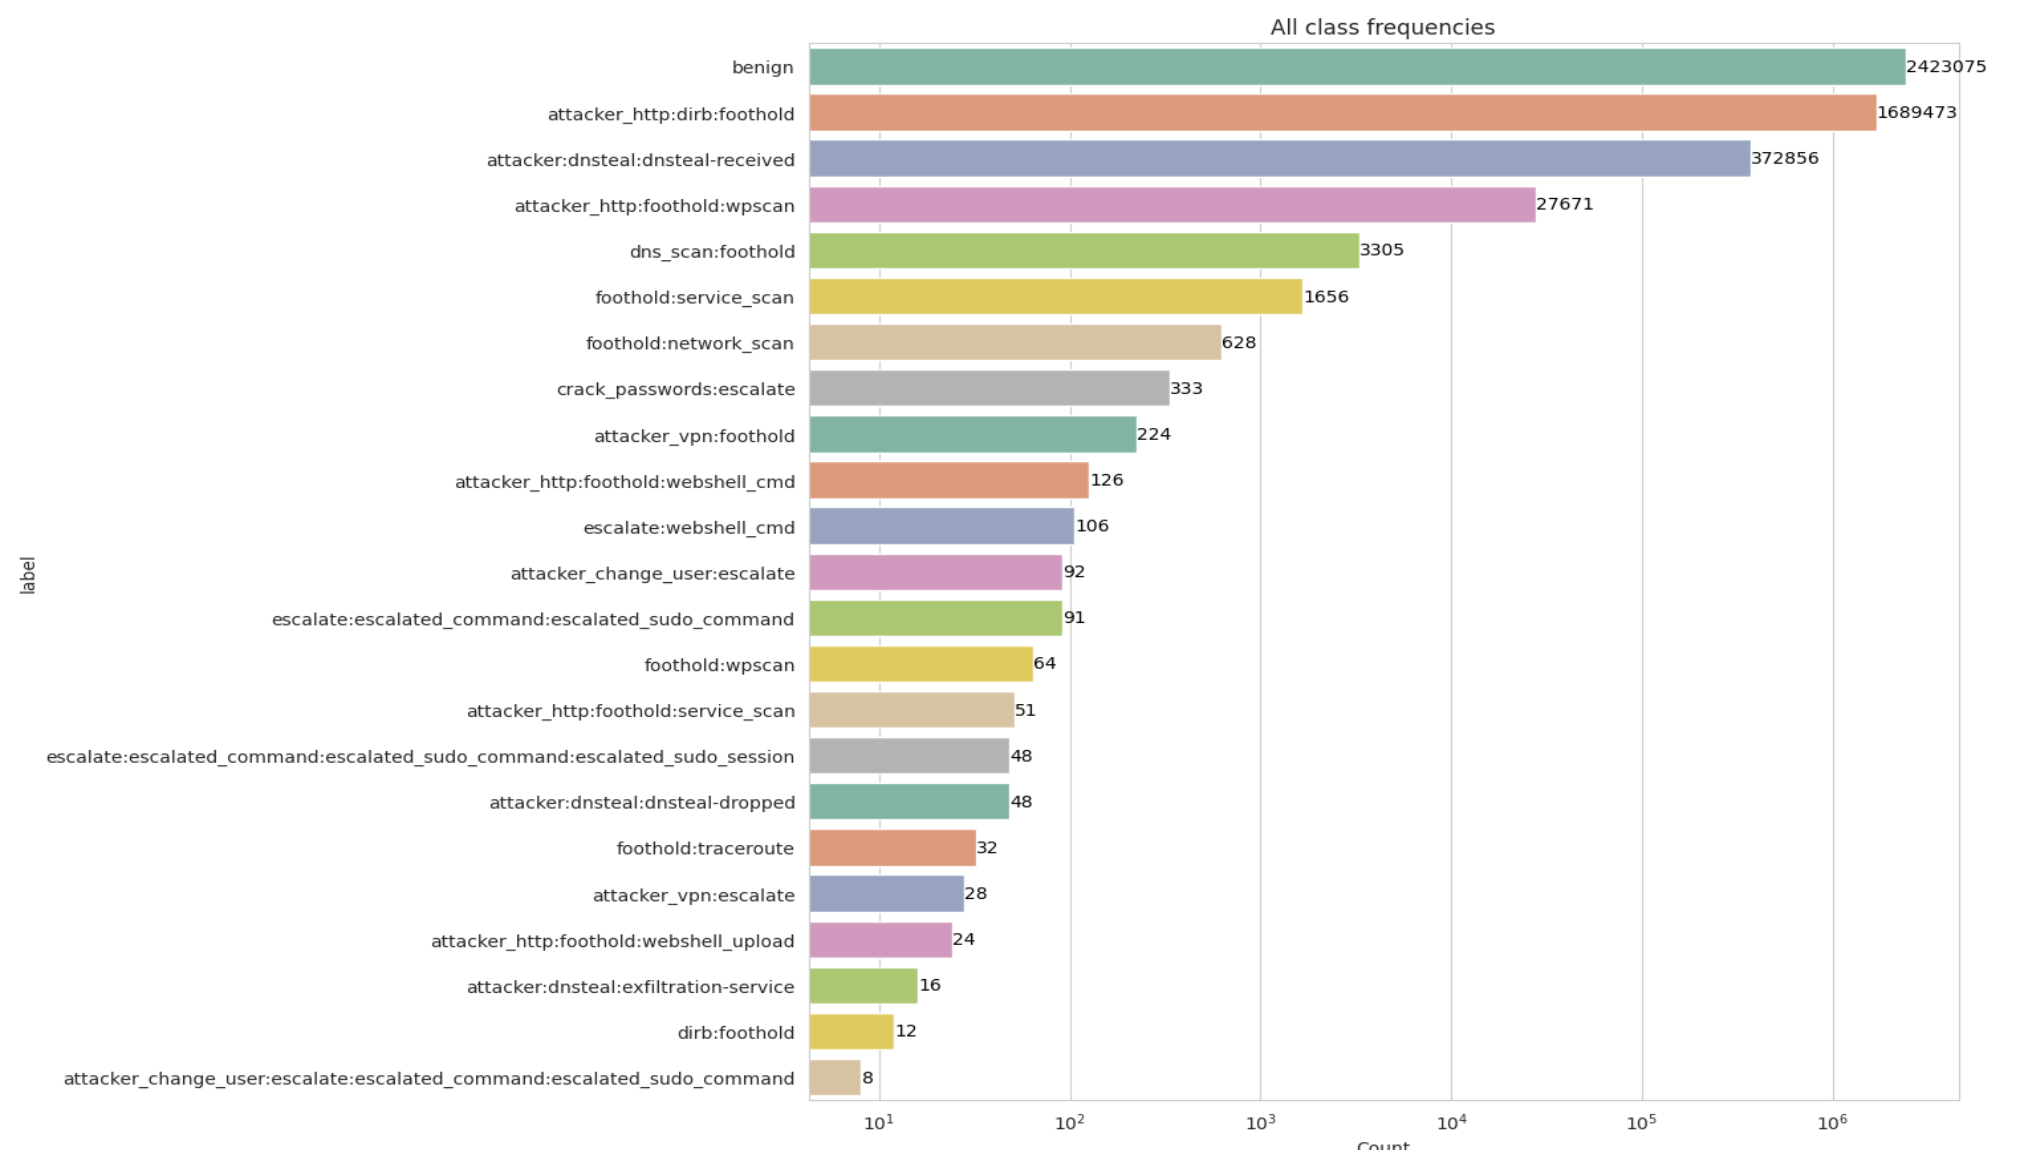
\includegraphics[width=0.8\textwidth]{label_counts.png}
    \caption{Label Counts (Log-Scaled X-Axis)}
    \label{fig:label_counts}
\end{figure}

Initially, we capped the maximum number of samples to 100,000 per class. Despite the imbalance, our model achieved impressive performance without the need for extensive data augmentation.

\subsection{Data Profiling and Label Consolidation}

The dataset originally comprised over 48 different types of network attacks. To streamline the modeling process and enhance the model's ability to generalize, we consolidated these attack types into six broader categories, as detailed in Section~\ref{sec:methodology}.

\section{Methodology}
\label{sec:methodology}

\subsection{Model Selection}

We utilized DistilBERT \citep{sanh2019distilbert}, a distilled version of BERT that offers faster performance while maintaining a high level of accuracy. DistilBERT is particularly suitable for inference on CPUs, making it practical for deployment in real-world settings.

\begin{figure}[htbp]
    \centering
    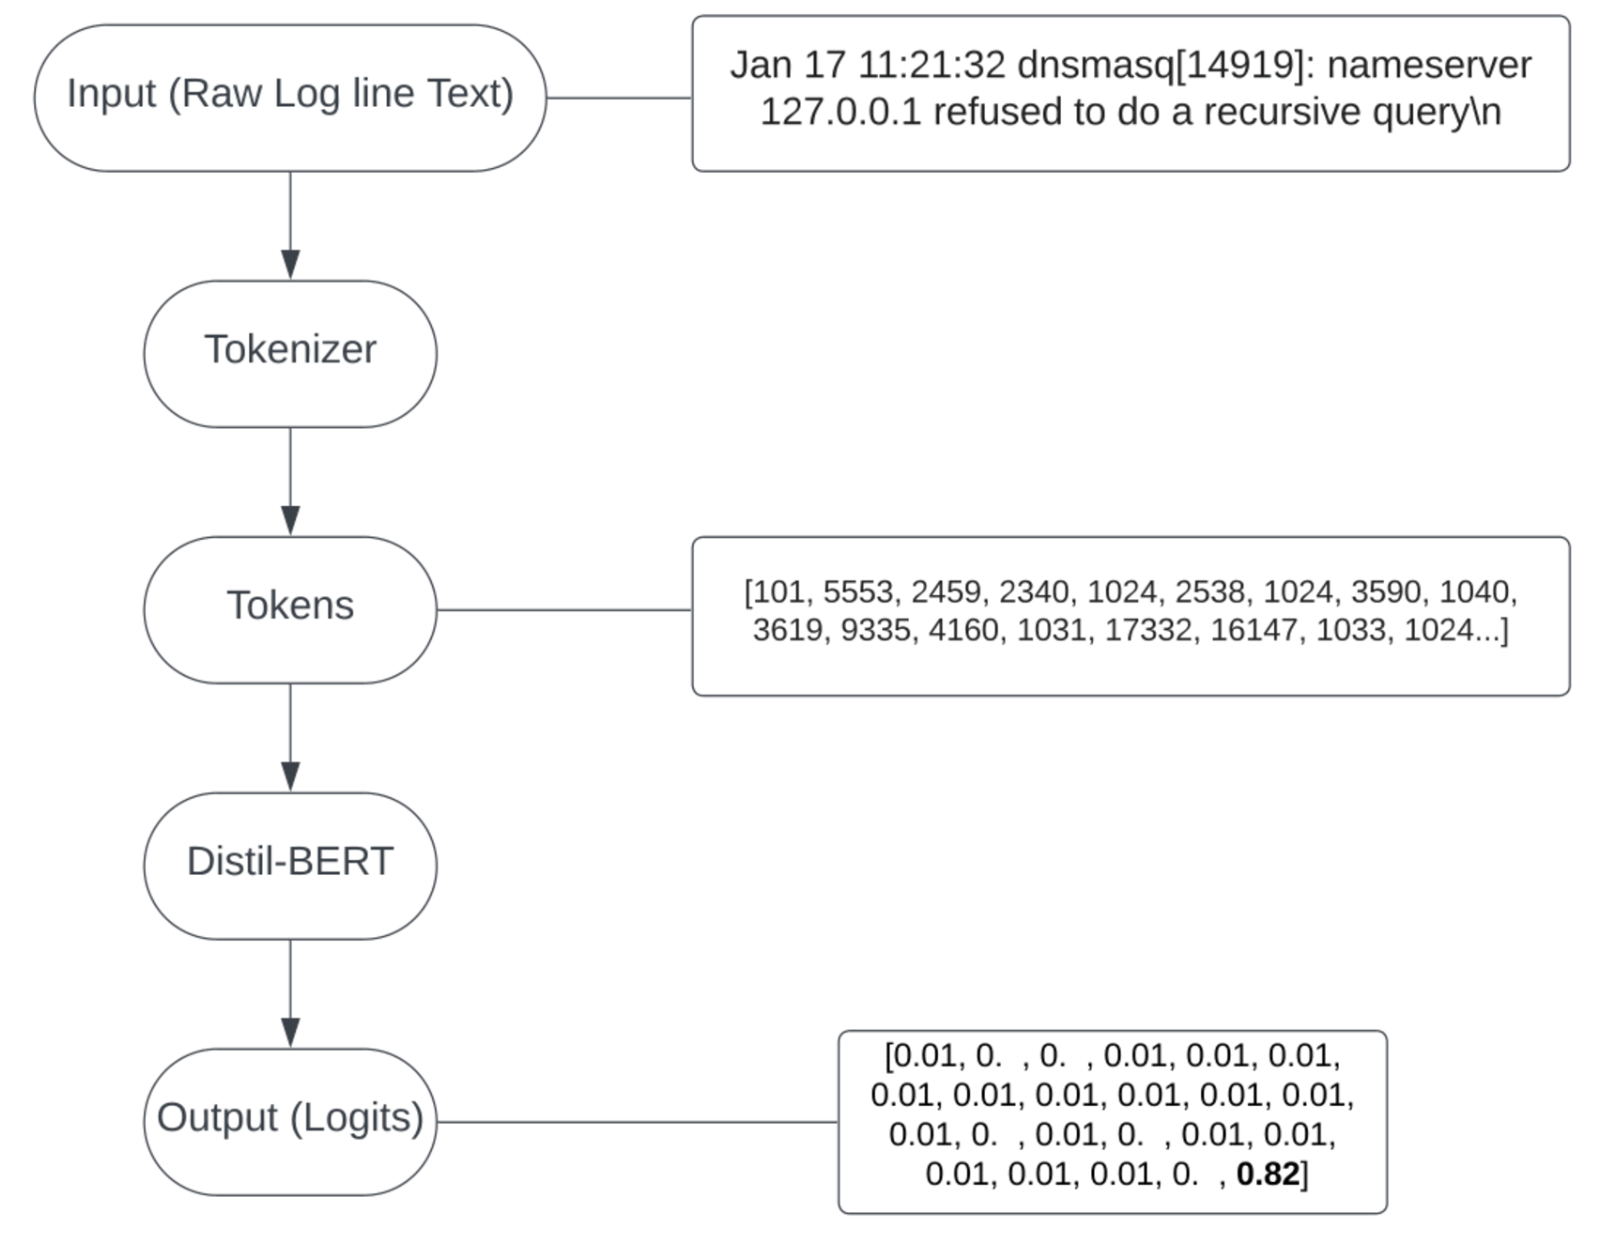
\includegraphics[width=0.6\textwidth]{distil_bert.png}
    \caption{DistilBERT Architecture}
    \label{fig:distil_bert}
\end{figure}

\subsection{Model Training}

We performed 5-fold cross-validation on the data and averaged the accuracies across the five confusion matrices. For computational efficiency, the models trained for the validation were limited to 10,000 samples from each label. To prevent data leakage, we used stratified sampling to create the training and test sets.

\subsection{Classification Strategy}

The model outputs logits for each class, representing the unnormalized log probabilities. We select the class associated with the highest logit value as the predicted class. The output logits can be interpreted as a likelihood of class selection, which can be used to adjust sensitivity and manage false positives through a threshold mechanism.

\begin{figure}[htbp]
    \centering
    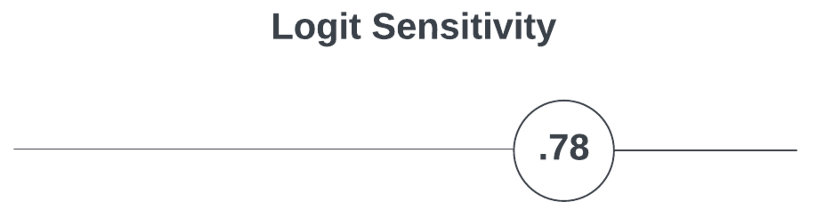
\includegraphics[width=0.7\textwidth]{logit_sensitivity.png}
    \caption{Logit Sensitivity Thresholding}
    \label{fig:logit_sensitivity}
\end{figure}

\section{Results}

\subsection{Model Performance}

The confusion matrix in Figure~\ref{fig:confusion_matrix} shows the average results from the classification on the five test sets. Despite the data imbalance, our model achieved outstanding results.

\begin{figure}[htbp]
    \centering
    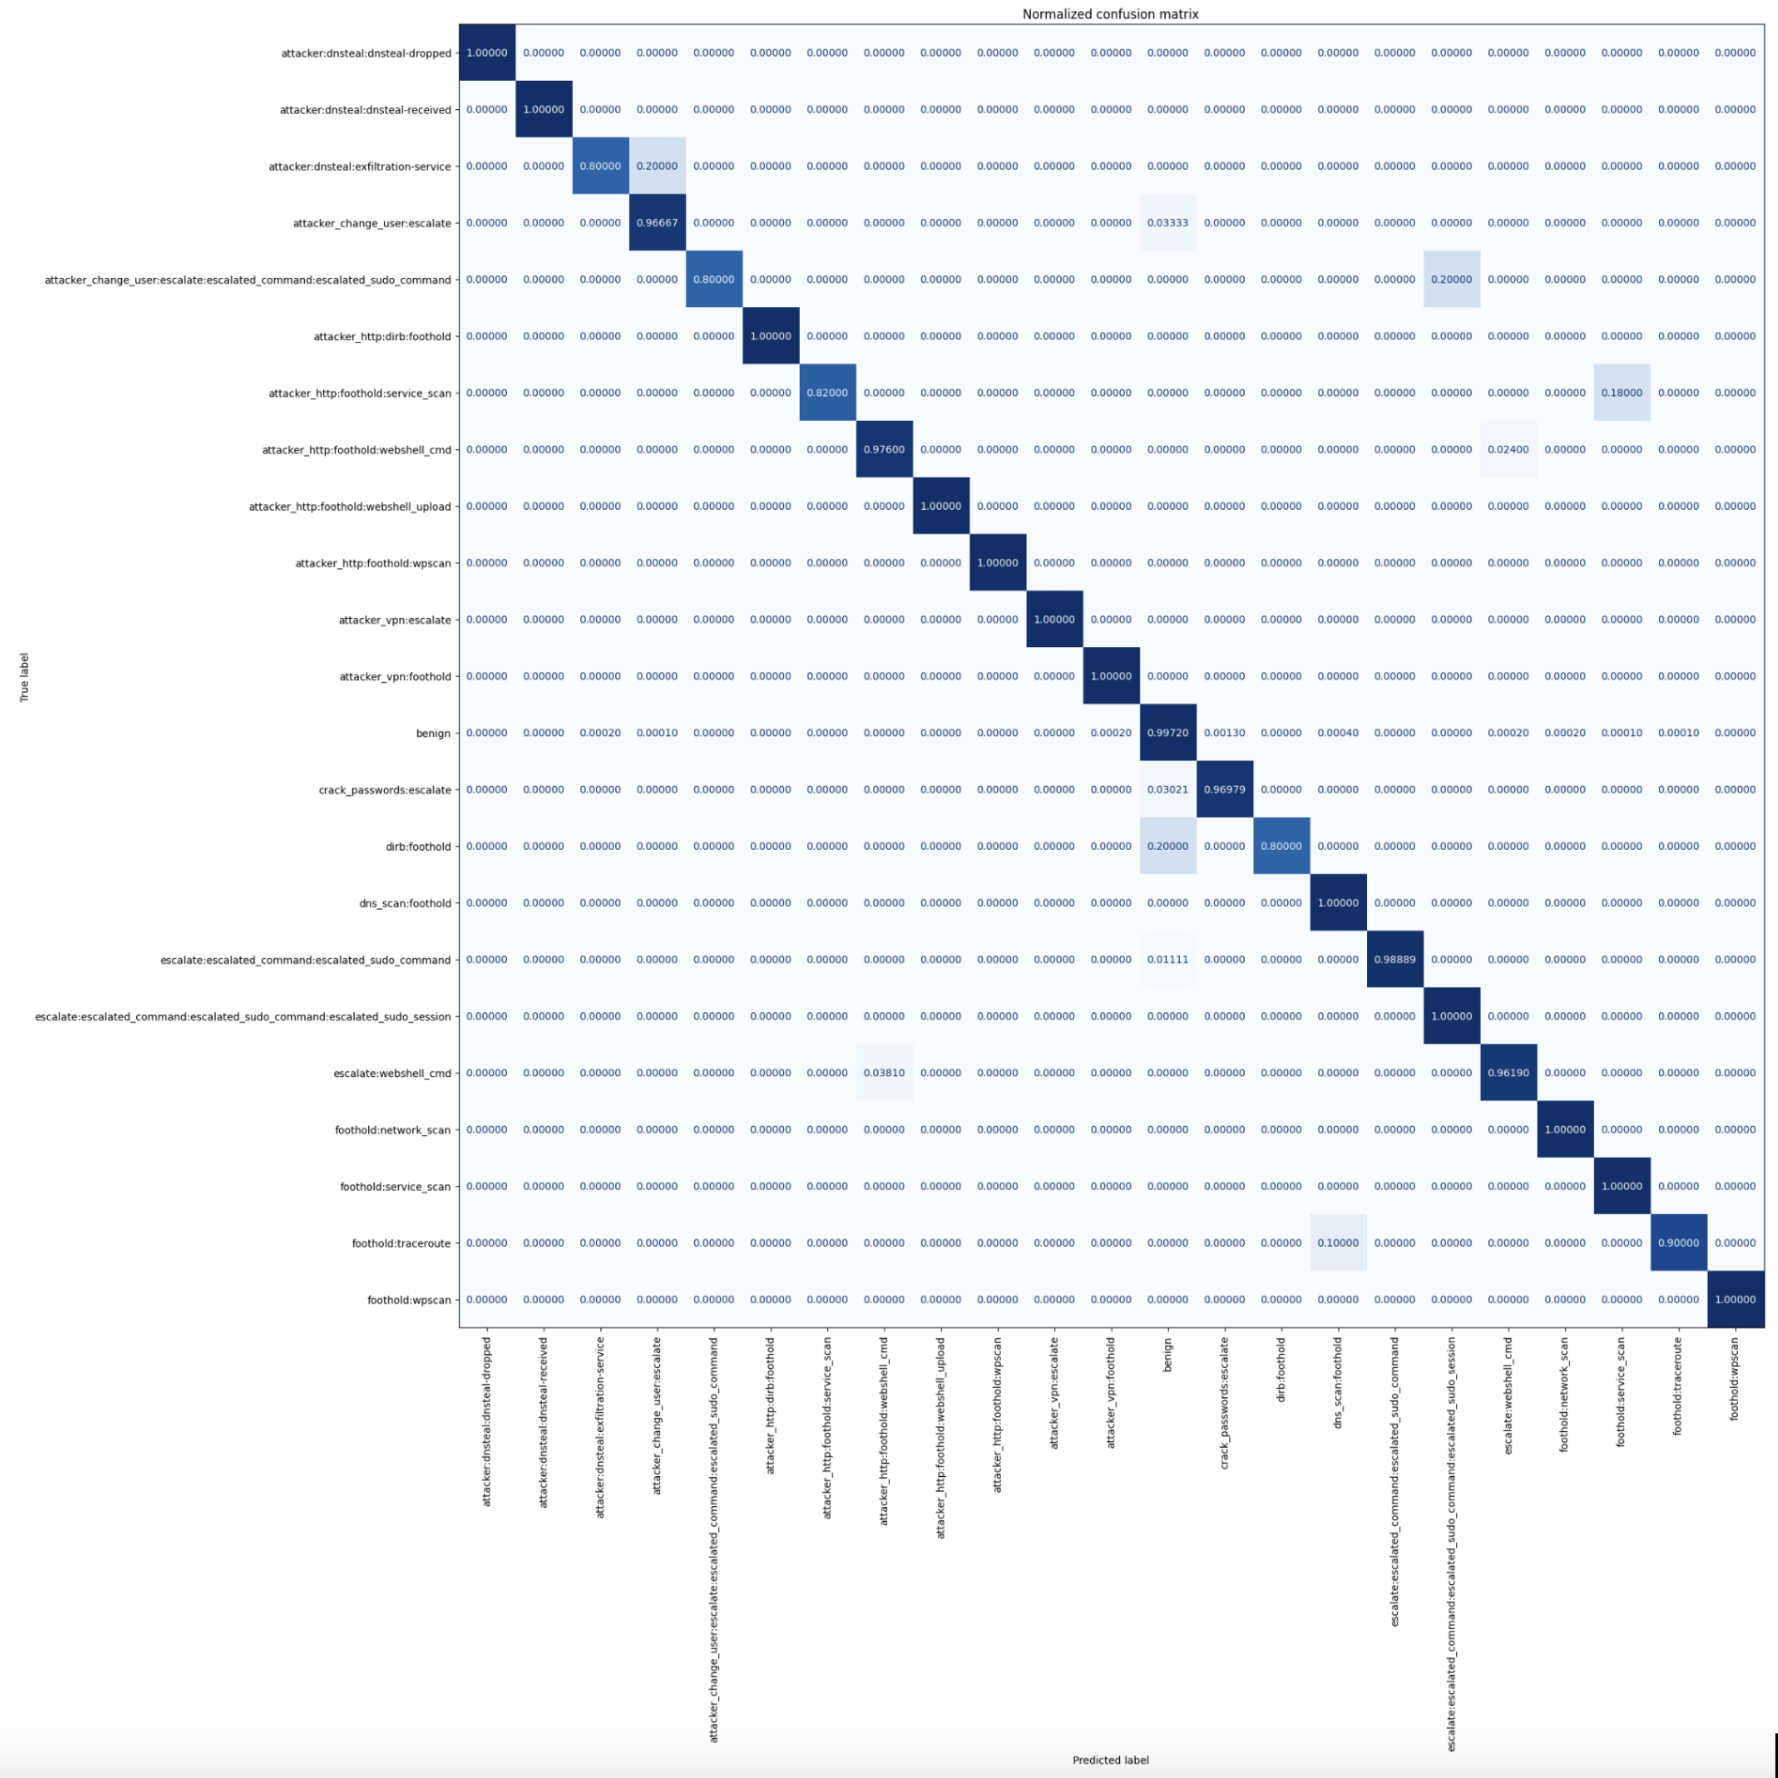
\includegraphics[width=0.8\textwidth]{confusion_matrix.png}
    \caption{Average Confusion Matrix from 5-Fold Cross-Validation}
    \label{fig:confusion_matrix}
\end{figure}

\subsection{Evaluation Metrics}

Our fine-tuned DistilBERT model achieved:

\begin{itemize}
    \item \textbf{Accuracy}: 99.7\%
    \item \textbf{Precision}: 99.6\%
    \item \textbf{Recall}: 99.5\%
    \item \textbf{F1-Score}: 99.6\%
\end{itemize}

These metrics indicate the model's high effectiveness in classifying network intrusion activities.

\subsection{Analysis}

The high classification accuracy demonstrates that treating log data as pseudo-natural language allows the model to capture intricate patterns and correlations. The model effectively distinguishes between benign and malicious log lines, even among classes with fewer samples.

\section{Implementation}

\subsection{Model Hosting}

The model is currently hosted on Hugging Face at:

\begin{center}
    \url{https://huggingface.co/isaacwilliam4/insyt}
\end{center}

This platform allows us to download the model, keep track of versions, and use the inference API to input our own log lines and see the model's predictions.

\subsection{Full-Stack Framework}

To enhance usability, we developed a Python package that can be installed to analyze log files and track network intrusions.

\begin{figure}[htbp]
    \centering
    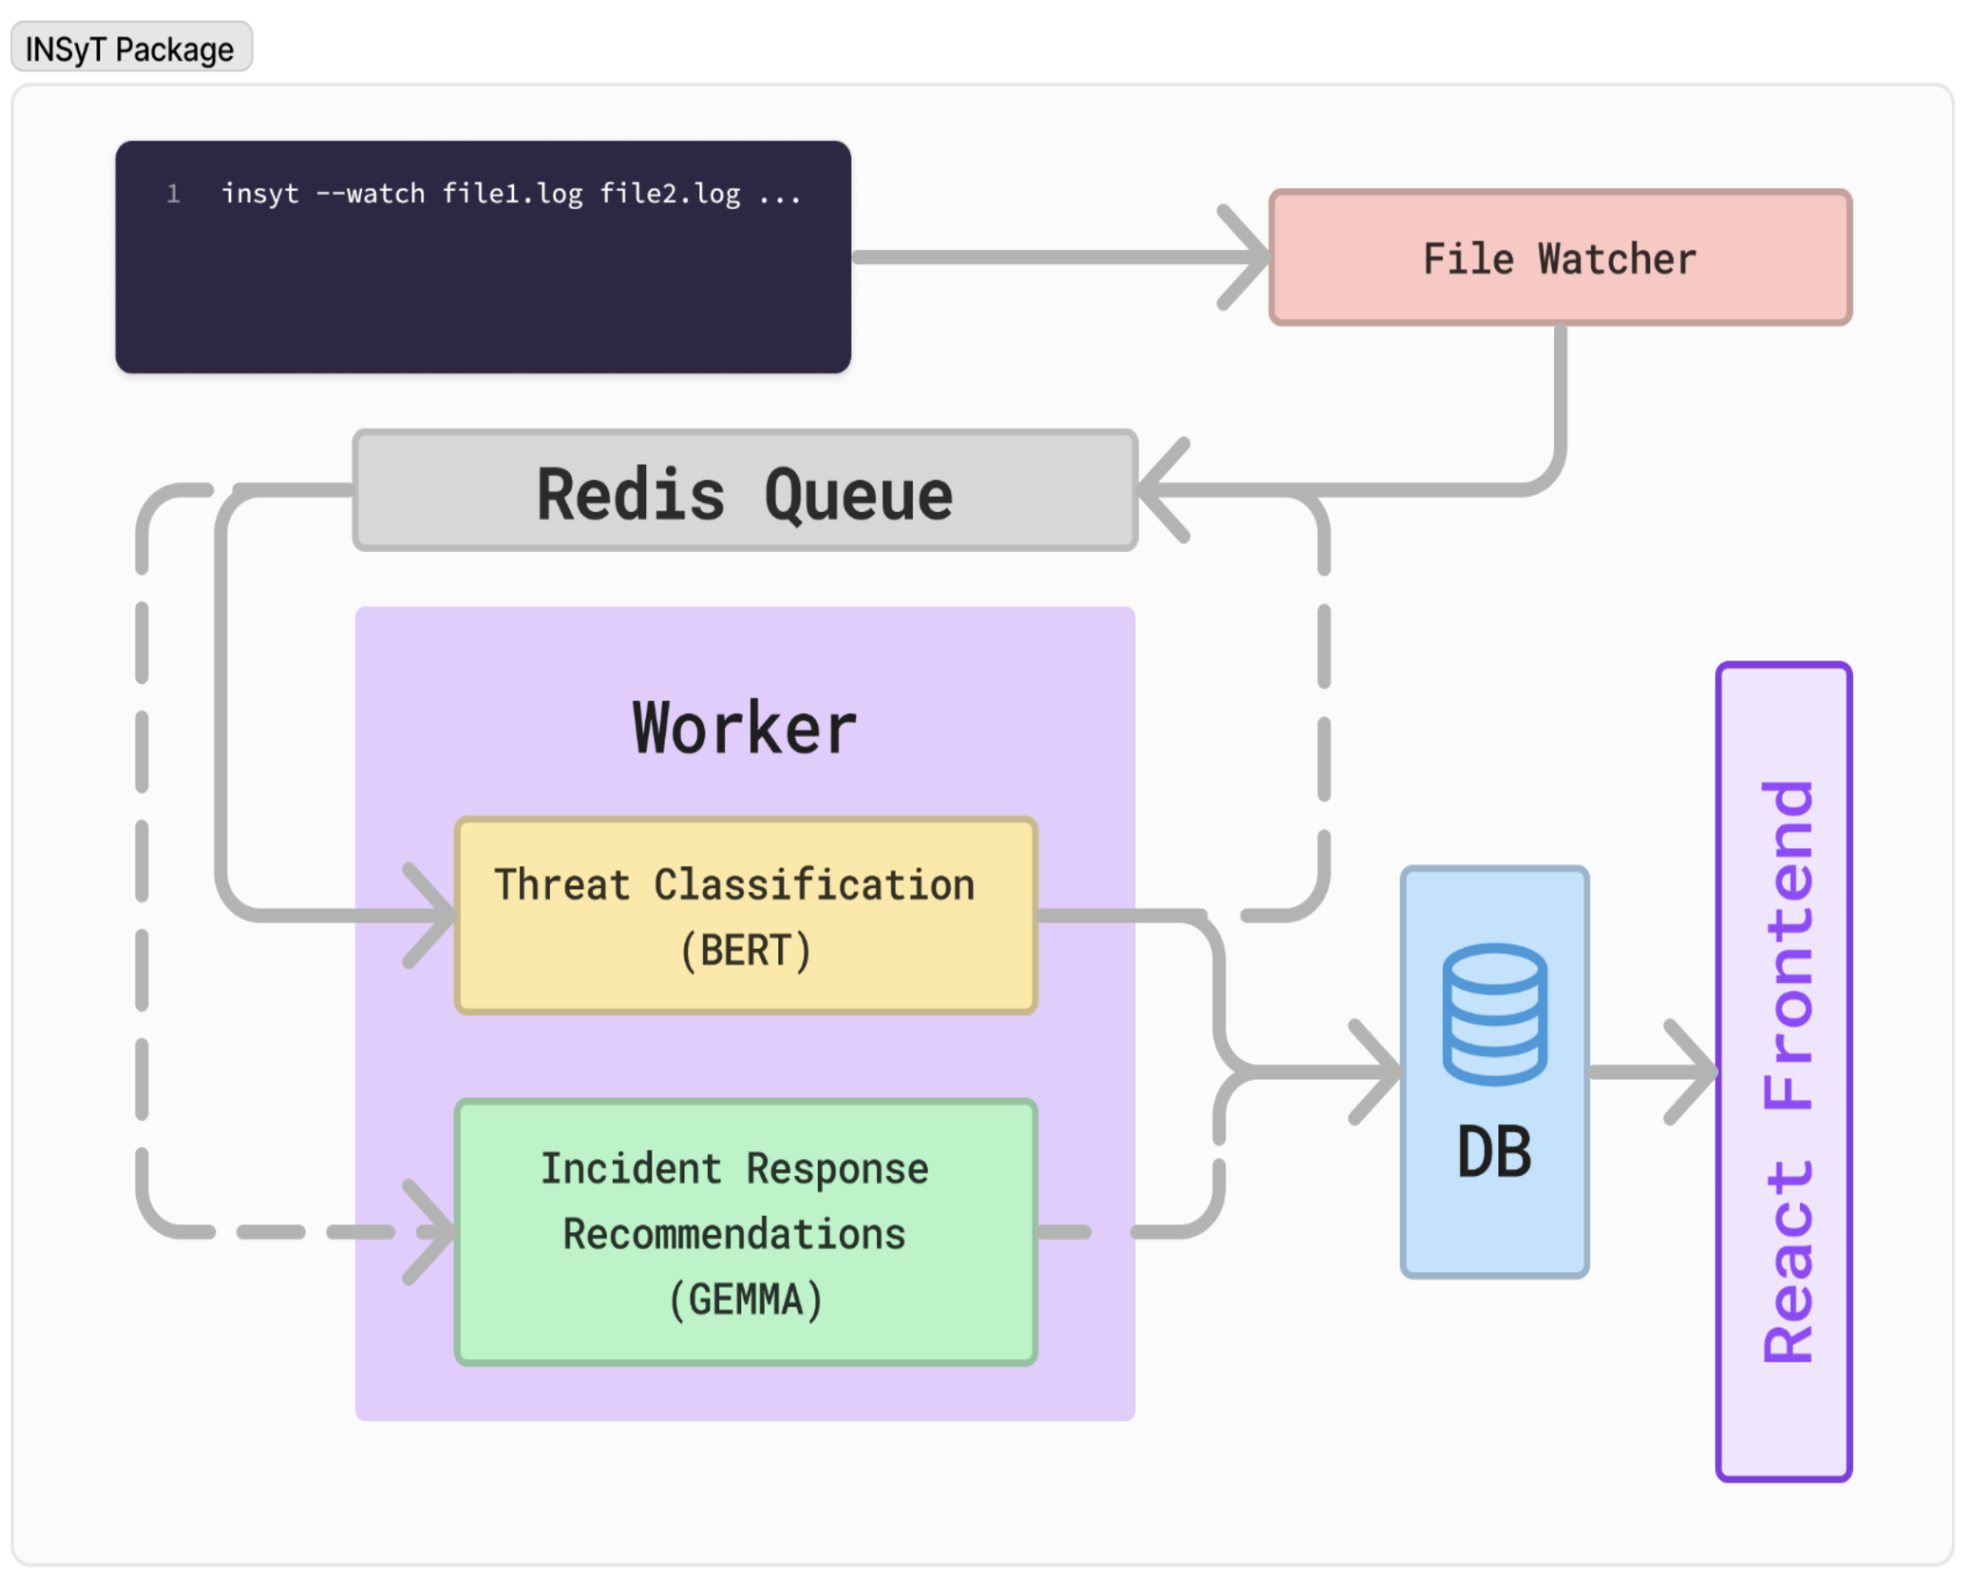
\includegraphics[width=0.8\textwidth]{insyt_package.png}
    \caption{NLP Framework for Network Intrusion Detection}
    \label{fig:insyt_package}
\end{figure}

\subsubsection{Workflow}

The package daemon operates in three steps:

\begin{enumerate}
    \item \textbf{File Watcher}: Monitors log files and queues new lines using Redis.
    \item \textbf{Worker Process}: Retrieves log lines from the queue, runs them through our classification model, logs results in a SQLite database, and re-queues lines identified as threats.
    \item \textbf{Threat Analysis}: Processes classified threats with Gemma, offers analysis and response recommendations, and loads analyses into the database.
\end{enumerate}

\subsection{User Interface}

We developed a React frontend that connects to the local database to display classification results. This interface allows users to:

\begin{itemize}
    \item Monitor real-time intrusion detection logs.
    \item Adjust sensitivity thresholds using a slider based on output logits.
    \item View detailed analysis and response recommendations.
\end{itemize}

\begin{figure}[htbp]
    \centering
    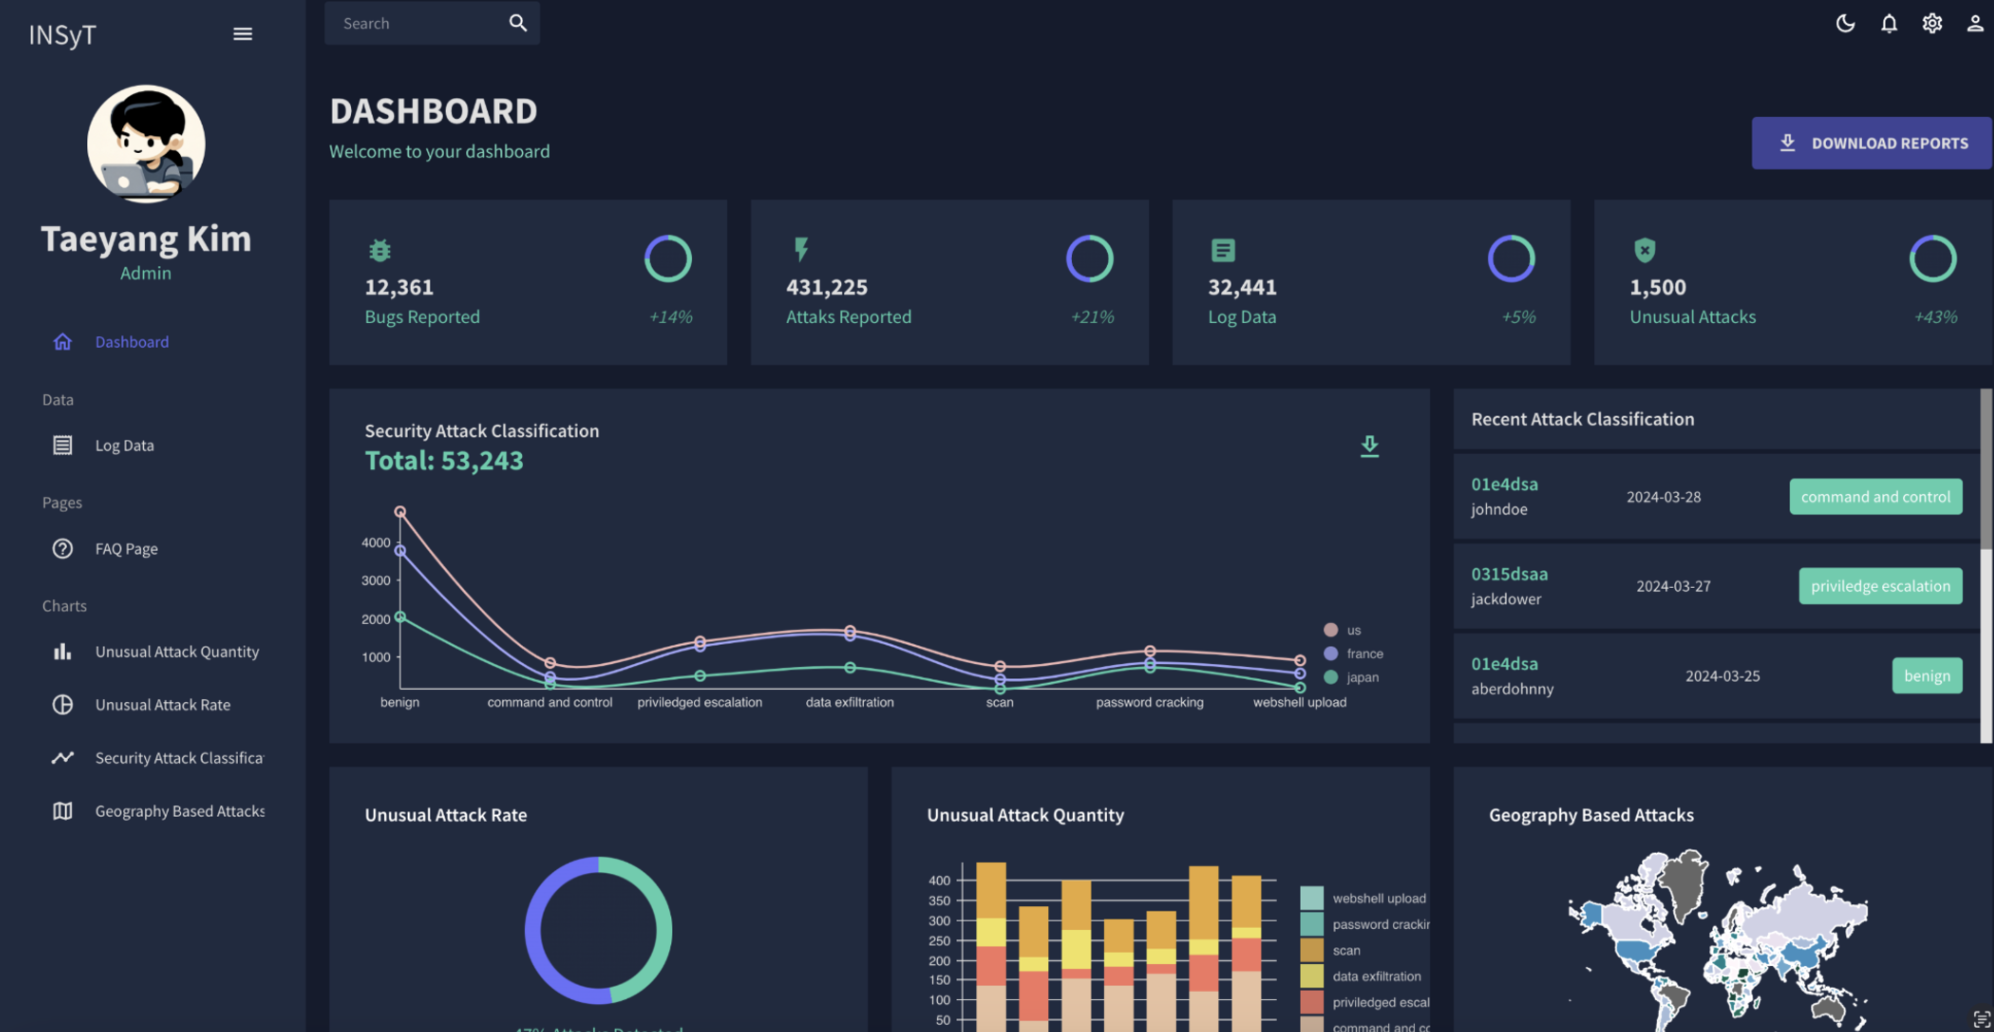
\includegraphics[width=0.8\textwidth]{react.png}
    \caption{React Frontend for Network Intrusion Detection}
    \label{fig:react}
\end{figure}

\section{Discussion}

\subsection{Impact and Benefits}

Our LLM-based NIDS offers significant advantages:

\begin{itemize}
    \item \textbf{High Accuracy}: Achieving 99.7\% accuracy reduces the risk of undetected intrusions.
    \item \textbf{Efficiency}: The model processes logs quickly and can operate effectively on CPUs.
    \item \textbf{Scalability}: Hosting on Hugging Face and using containerization allows for easy deployment and scaling.
\end{itemize}

\subsection{Challenges}

\begin{itemize}
    \item \textbf{Data Imbalance}: While we achieved high accuracy, further work could involve handling data imbalance more robustly, possibly improving performance on minority classes.
    \item \textbf{Tokenization of Log Data}: Fine-tuning the tokenizer was essential due to the pseudo-natural language of logs.
    \item \textbf{Model Generalization}: Ensuring the model generalizes well to logs from different systems remains an area for future work.
\end{itemize}

\subsection{Future Work}

\begin{itemize}
    \item \textbf{Data Augmentation}: Implement techniques to balance the dataset further.
    \item \textbf{Real-Time Deployment}: Optimize the system for high-throughput environments.
    \item \textbf{Extended Testing}: Validate the model on diverse datasets to assess generalizability.
\end{itemize}

\section{Conclusion}

We have developed a full-stack LLM network intrusion detection system that leverages advanced NLP techniques to analyze system and network logs as natural language. Our fine-tuned DistilBERT model achieved 99.7\% accuracy in classifying network intrusions into six major categories. The system offers significant improvements over traditional NIDS in terms of accuracy, adaptability, and cost-effectiveness.

This project demonstrates the potential of LLMs in cybersecurity applications and sets the groundwork for further advancements in intelligent threat detection systems.

\section*{Acknowledgments}

We thank Sandia National Laboratories, particularly Ryan Holt and Mike Reed, for their support and collaboration. We also acknowledge the contributions of the INSyT team members: Bronze Frazer, Taeyang Kim, Isaac Peterson, and Damon Tingey.

\bibliographystyle{plainnat}
\begin{thebibliography}{9}
\bibitem{databreachreport}
IBM Security and Ponemon Institute. (2023).
\newblock \emph{Cost of a Data Breach Report 2023}.
\newblock Retrieved from \url{https://www.ibm.com/security/data-breach}

\bibitem{traditionalnids}
Garcia-Teodoro, P., Diaz-Verdejo, J., Macia-Fernandez, G., \& Vazquez, E. (2009).
\newblock Anomaly-based network intrusion detection: Techniques, systems and challenges.
\newblock \emph{Computers \& Security}, 28(1-2), 18-28.

\bibitem{anomalyissues}
Sommer, R., \& Paxson, V. (2010).
\newblock Outside the closed world: On using machine learning for network intrusion detection.
\newblock In \emph{2010 IEEE Symposium on Security and Privacy} (pp. 305-316).

\bibitem{neuralnids}
Kim, G., Lee, S., \& Kim, S. (2014).
\newblock A novel hybrid intrusion detection method integrating anomaly detection with misuse detection.
\newblock \emph{Expert Systems with Applications}, 41(4), 1690-1700.

\bibitem{bert}
Devlin, J., Chang, M. W., Lee, K., \& Toutanova, K. (2019).
\newblock BERT: Pre-training of Deep Bidirectional Transformers for Language Understanding.
\newblock In \emph{Proceedings of NAACL-HLT 2019} (pp. 4171–4186).

\bibitem{sanh2019distilbert}
Sanh, V., Debut, L., Chaumond, J., \& Wolf, T. (2019).
\newblock DistilBERT, a distilled version of BERT: smaller, faster, cheaper and lighter.
\newblock \emph{arXiv preprint arXiv:1910.01108}.

\bibitem{landauer2022ait}
Landauer, M., Skopik, F., Frank, M., Hotwagner, W., Wurzenberger, M., \& Rauber, A. (2022).
\newblock AIT Log Data Set V2.0 (v2\_0) [Data set].
\newblock Zenodo. \url{https://doi.org/10.5281/zenodo.5789064}

\end{thebibliography}

\end{document}